% LaTeX 2e sinon rien !
\NeedsTeXFormat{LaTeX2e}

% C'est un rapport...
\documentclass[a4paper,11pt]{report}

% Style du document : personnalisé si disponible, sinon LaTeX par défaut
\newif\ifbglstyle
\IfFileExists{bglstyle.sty}{
  \usepackage{bglstyle}
  \bglstyletrue
}{
  \bglstylefalse
}

\ifbglstyle\else
  % Packages de base
  \usepackage[utf8]{inputenc}
  \usepackage[T1]{fontenc}
  \usepackage{ifpdf,textcomp,ae,aecompl,aeguill}
  \usepackage[margin=3cm]{geometry}

  % Commandes définies ici pour assurer la compatibilité avec le style perso
  \makeatletter
  \renewcommand{\title}[1]{\renewcommand{\@mytitle}{#1}}
  \newcommand{\@mytitle}{}
  \newcommand{\subtitle}[1]{\renewcommand{\@title}{\@mytitle\\#1}}
  \newcommand{\group}[1]{}
  \newcommand{\entity}[1]{}
  \makeatother

  % Si jamais le rendu du style LaTeX standard diffère légèrement du style
  % personnalisé, ça ne produira pas d'avertissement (overful/underful hbox)
  \sloppy
\fi

% Packages supplémentaires utilisés par ce document
\usepackage{graphicx,multicol}
\usepackage[french,english]{babel}

% Informations sur le document
\title{Jeu 3D en OpenGL/GLUT}
\author{Benjamin Gaillard, Nicolas Riegel}
\date{17 mai 2006}
\group{Master 1 RIA --- Option MIG}
\entity{\includegraphics[keepaspectratio,height=1.5cm]{images/ulp}}

% Hyperlinks
\ifpdf
  \usepackage[pdftex,bookmarks,bookmarksopen,bookmarksnumbered,%
              pdfstartview=Fit,pdfview=FitH]{hyperref}
  \makeatletter
  \hypersetup{%
    pdftitle  = {\@title},
    pdfauthor = {\@author},
    pdfborder = {0 0 0}
}
  \makeatother
  \usepackage{thumbpdf}
\else
  \usepackage[dvips]{hyperref}
\fi

% Redéfinition d'une information (pour la présentation)
\title{{\large Matériels et Interfaces Graphiques}\\Jeu 3D en OpenGL/GLUT}
\subtitle{Rapport}
\author{Benjamin \textsc{Gaillard}\\Nicolas \textsc{Riegel}}

% Commandes personnalisées
\newcommand{\ensp}[1]{\selectlanguage{english}#1\selectlanguage{french}}
\newcommand{\strong}[1]{\textbf{#1}}
\newcommand{\file}[1]{\ensp{\textsf{#1}}}
\newcommand{\var}[1]{\ensp{\textit{#1}}}
\newcommand{\type}[1]{\ensp{\texttt{#1}}}
\newcommand{\func}[1]{\ensp{\textsf{#1}}}
\newcommand{\class}[1]{\ensp{\textsf{#1}}}
\newcommand{\bs}{\textbackslash}


\begin{document} % Pas d'indentation pour cet environnement de base

\selectlanguage{french}
\maketitle
\tableofcontents



\chapter{Introduction}

\section{Choix du sujet}

Nous avons choisi la réalisation d'une application interactive de type navigation dans un monde en 3D.
C'est en s'inspirant d'un jeu existant, Wipeout, que nous est venue l'idée de faire ce jeu. Il consiste en une
course chronométrée avec un petit vaisseau qui vole le long d'un circuit.
Le sujet comporte plusieurs exigences :
\begin{itemize}
 \item l’utilisation exclusive d’OpenGL avec comme système de fenêtrage GLUT (utilisé uniquement pour ouvrir une fenêtre et un contexte
         OpenGL pour récupérer les évènements) ;
 \item il est imposé d’utiliser des modèles 3D et des textures 2D ;
 \item il est imposé d’utiliser l’éclairage OpenGL (donc au moins une source de lumière OpenGL).
\end{itemize}

\bigskip
Le jeu devra aussi fonctionner correctement sur les machines de la salle C310 sous Linux.
Il est important et imposé que le jeu comporte des éléments de navigation 3D à l’aide des touches de clavier et/ou de la souris.
L’environnement devra être modélisé en 3D à l’aide de polyèdres. Les textures peuvent être récupérées sur le web ainsi que les modèles 3D (s’il
y a lieu). Les éléments actifs (personnages ou certains objets par exemple) pourront être modélisés soit explicitement en 3D soit sous la forme
de \textit{billboards}. On intégrera des objets tri-dimensionnels animés. Ces objets pourront répondre à un stimulus extérieur (suite à une action de
l'utilisateur) ou avoir une autonomie propre.

\section{Compilation et exécution}

La projet utilisant les GNU Autotools, sa compilation se fait de la même
manière que la plupart des applications Unix. Placez-vous dans la racine des
sources du projet et tapez :

\begin{verbatim}
./configure [options...]
make
\end{verbatim}

Puis, éventuellement, \verb!make install! pour l'installer dans la hiérarchie
spécifiée au script \verb!configure! (\file{/usr/local} par défaut). Pour le
lancer, tapez \verb!podz! si vous l'avez installé, on \verb!src/podz! si vous
souhaitez l'exécuter directement depuis le répertoire des sources.

\bigskip
Dans ce programme, vous pourrez utiliser les touches suivantes :
\begin{description}
	\item[Échap ou Q :] Quitte le jeu.
	\item[Flèche haut :] Accélère.
	\item[Flèche bas :] Freine jusqu'à l'arêt.
	\item[Flèche droite ou gauche :] Tourner à droite ou à gauche.
	\item[F :] Met ou sort du mode plein écran.
	\item[T :] Désactive les textures.
	\item[L :] Désactive les lumières.
	\item[Espace ou P :] Met en pause.
\end{description}

\section{Informations supplémentaires}

Ce jeu a été réalisé intégralement en anglais (à quelques commentaires près)
afin qu'il puisse éventuellement être repris et amélioré par d'autres
personnes si nous mettons à disposition notre projet.

La compilation a été testée avec GCC sous Linux et Microsoft Visual C++%
\footnote{Version gratuite disponible sous l'intitulé \og Microsoft Visual C++
Express Edition\fg} sous Windows. Elle devrait également se dérouler
correctement sous Mac OS X, mais ne possédant pas de Mac, nous n'avons pas pu
tester cette possibilité. Nous nous sommes basés sur des renseignements
trouvés sur Internet pour une compatibilité avec ce système d'exploitation.


\chapter{Structure du programme}

La fonction \func{main()} est dans le fichier \file{Application.cpp}. Elle ne
fait qu'instancier la classe \type{Application} qui contient les objets
principaux et lancer la boucle principale de GLUT.

GLUT utilise un mécanisme de \textit{callback} pour informer l'application des
événements qui se produisent. L'interfaçage avec nos classes se fait en
utilisant des variables statiques contenant les instances des classes qui
géreront les événements. Les fonctions de \textit{callback} les utilisent pour
appeler les méthodes correspondantes. Cela nous permet d'interfacer GLUT avec
notre projet orienté objet.

\section{Interfaçage avec GLUT}

GLUT permet de gérer plusieurs sources d'évéments. Nous avons classés ceux qui
nous intéressaient en trois catégories, chacune représentée par une classe.

\section{L'affichage : classe Display}

Cette classe contient tout le système de gestion d'affichage. Lors de son instanciation, on initialise la fenêtre GLUT. Pour passer en mode plein
écran, on utilise la fonction \func{glutEnterGameMode()}. Malheuresement cette fonction nous oblige à relancer toutes les fonctions de rappel GLUT
ainsi qu'à recharger toutes les textures. Pour l'affichage de texte nous avons créé une petite fonction dans la classe \type{Display} : \func{DisplayText()}.
Cette fonction prend en paramètre le texte et les coordonnées, et éventuellement la taille.

Les différents objets susceptibles d'avoir un effet avec l'affichage sont,
après instanciation de cette classe, enregistrés (ils sont stockés dans une
liste). Les classes de ces objets dérivent toutes de la classe abstraite
(virtuelle) \type{Object}.

Lors d'un événement demandant l'affichage de la scène, trois méthodes sont
appelées successivement, et chacune pour tous les objets :
\begin{itemize}
  \item mise au point de la matrice de \textit{modelview} ;
  \item paramétrage des lumières OpenGL ;
  \item finalement, affichage des objets 3D.
\end{itemize}

\section{La gestion du clavier : classe Keyboard }

Pour pouvoir gérer les touches multiples (par exemple avant et droite en même temps), on a mis un booléen pour chacune des 4 touches de direction. On définit
les 3 fonctions de callback GLUT qui gèrent l'appuie d'une touche normale, l'appuie d'une touche spéciale et le relachement d'une touche spéciale. Pour
cela on utilise la même astuce que précédemment. Les deux dernières mettent simplement à jour les booléens. C'est avec le timer que l'on viendra regarder
quelles touches sont enfoncées ou non et agir en conséquence.

\section{Le timer : classe Timer}

C'est dans cette classe que vont être gérés les différents états du jeu, le chronomètre, ainsi que les déplacements du vaisseau. Pour le timer, on utilise
la fonction GLUT. Lorsque le timer expire, on le réarme, puis selon l'état on affiche le message correspondant ou on déplace le vaisseau.


\chapter{Rendu 3D}

\section{Classe de base Object}

Les objets qui vont pouvoir être affichés ont tous une classe qui dérive de
la classe \type{Object}. Cette classe définit les méthodes virtuelles appelées
par \type{Display} ainsi que deux fonctions permettant de dessiner un triangle
et un quadrilatère de manière simple (calcul de la normale, coordonnées de
texture automatiques\dots).

Le vaisseau a été modélisé \og à la main\fg{}, c'est-à-dire que nous n'avons pas utilisé de logiciel de modélisation, ni de modèle trouvé sur
internet. L'affichage du vaisseau utilise les fonctions \func{DrawQuad()} et \func{drawTriangle()} qui sont définies dans la classe \type{Object}.
Pour celà on procède par héritage. De la même manière, toutes les classes qui représenteront des objets 3D hériteront de la classe \type{Dessin}. C'est
le cas par exemple de la classe \type{Circuit}. Ces deux fonctions prennent en paramètre respectivement 4 et 3 points, un numéro de texture et éventuellement
les coordonnées d'affichage de la texture. La fonction met aussi en place les normales des polygones.

\section{Textures : classe Texture}

La gestion des textures se fait avec la classe \type{Texture}. Elle permet de
charger des images au format BMP (format brut non compressé) dans la mémoire
de la carte graphique. La méthode \func{Select} permet de sélectionner une
textures pour les opérations graphiques courantes.

\section{Objets 3D du jeu : classes Cube, Circuit et Vehicle}

Ces trois classes redéfinissent la méthode virtuelle d'affichage de la classe
Object. Certaines redéfinissent aussi la méthode de paramétrage des lumières
et Vechicle celle de placement de la caméra (matrice de \textit{modelview}).
Ces trois classes sont :
\begin{itemize}
  \item \textbf{\type{Cube} :} c'est un cube géant englobant toute la scène et
	qui affiche un décor au moyen de 6 textures, une par face (cet objet
	n'étant pas influencé par la lumière) ;
  \item \textbf{\type{Circuit} :} cette classe permet entre autre d'afficher
	le circuit chargé en mémoire ;
  \item \textbf{\type{Vehicle} :} celle-ci définit les lumières avant du
	vaisseau ainsi que son desssin, en plus d'autres fonctions.
\end{itemize}

\section{Listes d'affichage}

La classe \type{Object} stocke les commandes OpenGL de paramétrage des
lumières et d'affichage dans des listes d'affichage (\textit{Display List}).
Cela ne concerne évidemment que les commandes qui sont toujours les mêmes et
pas celles qui varient comme l'affichage d'informations textuelles sur le jeu
en cours.

L'avantage d'utiliser ces listes est d'accroître les performances générales
du programme puisqu'il n'est dès lors plus nécessaire de faires des calculs
pour obtenir les coordonnées des objets à afficher. Cela est particulièrement
intéressant pour la classe \type{Circuit} qui fait des calculs vectoriels
pour l'affichage.


\chapter{Le moteur de jeu}

\section{Classes utilitaires}

Afin de (grandement) faciliter la programmation des classes liées au moteur du
jeu, deux classes représentant des objets génériques. Il s'agit des classes :
\begin{itemize}
  \item \textbf{\type{Vector} :} opérations sur les vecteurs à trois
	dimensions (addition, produit vectoriel, mise à l'échelle, rotation,
	normalisation\dots) ainsi que la surcharge des opérateurs
	correspondant pour une meilleure facilité d'utilisation ;
  \item \textbf{\type{Basis} :} un repère dans un environnement 3D (origine
	et vecteurs unitaires), utilisé pour faire des changements de repère
	dans l'espace (utilisation d'une matrice de transformation et de son
	inverse).
\end{itemize}

\section{Les données du circuit}

La classe \type{Circuit} charge et stocke les informations relatives au
circuit. Pour construire un circuit, elle lit depuis un fichier les points de
l'espace par lesquels il passe, ainsi qu'une normale indiquant l'inclinaison
du circuit à ce point.

Au moyen d'une méthode d'interpolation, les points intermédiaires sont
calculés et à chacun un repère (classe \type{Basis}) est associé, indiquant
donc quatre informations sur ce point : sa localisation (origine) et trois
vecteurs unitaires qui sont : la tangente, la normale et un vecteur allant
vers le bord (côté).

Cette classe nous situe sur le circuit en utilisant une valeur appelée
\var{position} : il s'agit de la distance que l'on aurait parcourue si l'ont
était toujours resté exactement au centre de la piste. En utilisant une telle
valeur, la classe \type{Circuit} est capable de donner un repère (par
interpolation) dans l'espace.

\begin{center}
\noindent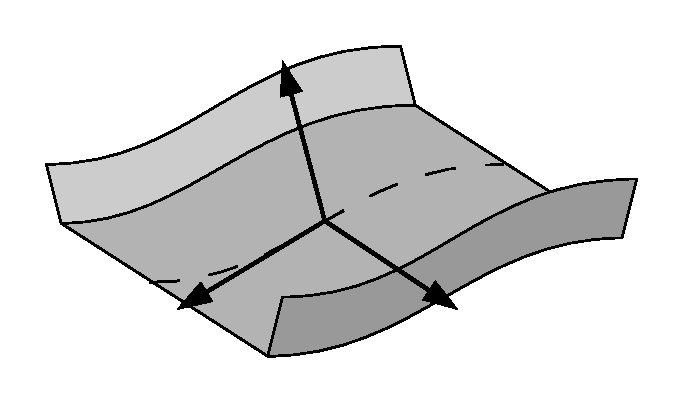
\includegraphics[keepaspectratio]{schemas/basis}
\end{center}

\section{Le vaisseau}

La classe \type{Vehicle} s'occupe de tout ce qui touche le vaisseau que le
joueur contrôle. Ses méthodes sont appelées par la classe \type{Keyboard} pour
réagir aux événements clavier de l'utilisateur. Elle est aussi responsable
de gérer la physique grâce à une méthode appelée périodiquement par le timer.

C'est la classe la plus complexe car elle effectue beaucoup d'opérations
vectorielles et de changement de base.


\chapter{Conclusion}

Ce projet nous a permis d'approfondir nos connaissances dans le langage C++ acquises l'année dernière, ainsi que dans le fonctionnement
d'OpenGL. Même si la programmation OpenGL n'est pas très adaptée au C++, nous avons réussi à nous débrouiller. Concernant le choix du
jeu, nous avons essayé de redonner vie à un jeu qui nous a passionné durant notre jeunesse, même si nous n'arrivons pas tout à fait
à la qualité du Wipeout original. Nous avons aussi voulu insister sur la jouabilité et non pas uniquement sur la beauté des graphismes.
Bon amusement !

\end{document}
